\documentclass[11pt,a4wide]{article}
\usepackage{a4wide}
\usepackage{graphicx}
\usepackage{float}
\begin{document}

\section{Introduction}
\subsection{Identification}
\indent The Specification and requirements document for the Linux Embedded Automotive Dashboard (LEAD) project defined by the client, University of Glasgow Racing Team. 

\section{Problem Definition}
University of Glasgow Racing Team (UG Racing) is in the process of building a formula type racing car for competition. The team requires new designs for several components of the new version of their car, as part of this the team has been subcontracted to replace the existing monochrome dashboard display with a new multifunctional colour USB display. The sensors and actuators in the car provides information about their state through an onboard Control Area Network Bus (CAN BUS), this data will be interpreted by the dashboard system to provide useful output to the driver.

\section{System Specification}
Following a discussion with the client a formal technical specification has been defined as follows
\begin{itemize}
	\item The following information must be displayed on the screen, speed, rpm, fuel, gear position, and warning indicators from data provided by the onboard CAN Bus.
	\item The display should be configurable through buttons on the display frame to allow a user to change units of measurement (i.e. mph to kph).
	\item The display should be easy to read preferably using a high contrast colour scheme, to be legible and clear from the driving position.
	\item The system should include a diagnostic menu to provide information about the other sensors on the CAN Bus.
	\item The system should include, if possible, a CAN Bus packet data logger.
	\item The CAN Bus interface should be compliant with ISO Standard 11898 (CAN Compliant)
\end{itemize}

\section{Constraints}
The client set some limitations on some factors of the system, primarly:
\begin{itemize}
	\item Power consumption, below 1.5A (including screen power)
	\item Scaling, Limited size, should fit in the dashboard allocated space.
	\item Robustness, The final system should be weather and vibration proof. It also should be robust to misuse (i.e. prevent misconnection).
\end{itemize}

\section{Design}
\subsection{Component Selection}
\subsubsection{Main Controller}
The proposed solution uses a Computer On Module (COM) designed by a company called Gumstix, the design will utilise the Overo Earth edition due to its relatively low price and appropriateness for the purposes of this project.
This module has been selected due to the following characteristics:
\begin{itemize}
	\item Compatible with GNU/Linux Operating System
	\item USB Host and On-The-Go ports are provided
	\item Communication to external devices through different protocols, including SPI
	\item A large number of General Purpose Input/Output pins
	\item A high processing power -- 600MHz
	\item A lower power consumption -- 250mA at 4V
	\item Provides commercial expansion board designs to facilitate the design of custom expansion boards.
\end{itemize}
The team looked into other alternatives like the Arduino which is popular at the moment for hobbbyist. However, the processing power is limited to a 16Mhz clock, it also does not have built-in support for USB and the amount of RAM provided is not enough to store a 24bit depth 800x480 image buffer (1.125MB). Another alternative was the BeagleBoard which provides a omap 3530 at 600MHz but the peripheral interfaces provided are not required for our purposes and like the gumstix CAN is not supported.

\subsubsection{CAN Interface}
The CAN Interface will be provided by a S08DZ60 Freescale microcontroller and a NXP TJA1040 transceiver. By using a co-processor like the S08DZ60 to receive and send the CAN packets we will be able to do post processing and filtering of the incoming packets, the current design of the circuit uses the SPI provided by both this microcontroller and the gumstix to transfer the packets. This microcontroller has been used because a 32 pins package is provided and therefore will limit the area of the PCB and facilitate the soldering process.\\
\\
The TJA1040 transceiver will be used to provide enough current to drive the CAN Bus and has been choosen as it is relatively simple to use in a design, it also provides sleep mode in case the CAN interface is not used and is well documented for its usage with the S08DZ60 family microcontrollers.\\
\\
The logic levels used by the gumstix and the S08DZ60 are different, and therefore a SN74LVC16T245 from Texas Instrument will be used to convert logic levels from 1.8V to 5.0V and vice versa.
\\
The first idea of implementation of the CAN interface was to used a microchip MPC2551 and MPC2515 however this can controller has a limited input and output buffers of only two packets therefore the gumstix would have to be interrupted really often to retrieve the data from the controller and therefore reduce the overall performance of the system.

\subsubsection{FTDI Communication}
To provide an easy way of communicating and configuring the system on the gumstix a FTDI232 chip will be used to provide serial communication through a USB connection.

\subsubsection{Screen}
The USB screen provided by the client will be used as the output for the dashboard and requires two USB ports for data and power. The model provided is the lilliput UM-70C but the interface used for the communication is a standard displaylink connection therefore any screen using this standard would be able to be used without any hardware or software change.

\subsubsection{Hardware Design Overview}

\begin{figure}[H]
\centering
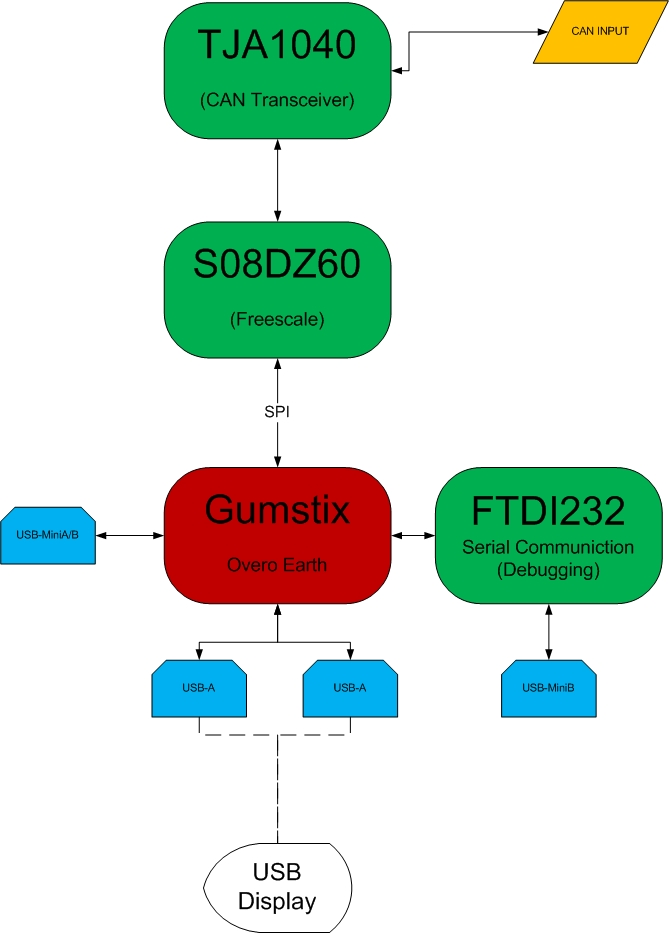
\includegraphics[scale=0.4]{High_Level_Schematic.jpg}
\caption{Hardware Design Overview}
\label{fig:hard_overview}
\end{figure}

\subsection{Software Selection}
\subsubsection{Operating System}
The team decided to use the GNU/Linux operating system as foundation for developement and deployment of the software as it provides compatibility with the screen DisplayLink protocol, and it increases the level of abstraction between the hardware and the software design therefore increasing the productivity and allowing further improvements or modifications to the application a simple development process.

\subsubsection{Proposed Solution}
The software will be developed using C programming language a X11 display server for Graphical User Interface (GUI) and SPI to retrieve the data from the CAN Bus through the S08DZ60 microcontroller.

\begin{figure}[H]
\centering
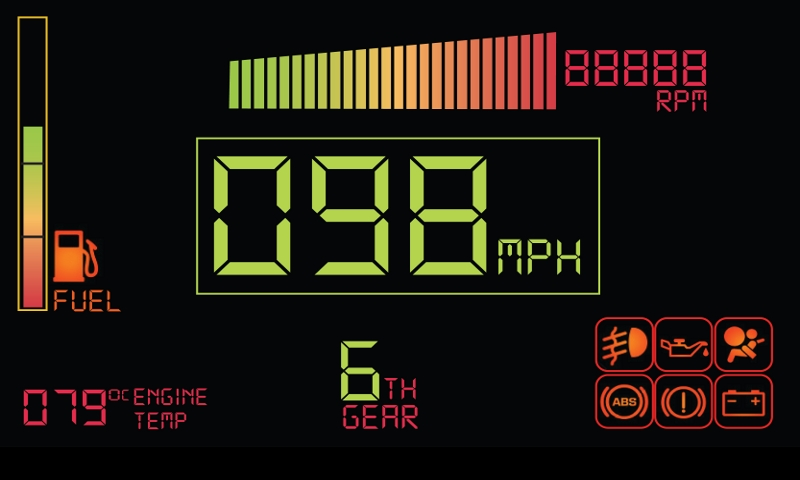
\includegraphics[scale=0.5]{dashboard-1_800x480.jpg}
\caption{Dashboard User Interface Prototype}
\label{fig:dash_proto}
\end{figure}

\section{References}
\begin{itemize}
	\item Current DashBoard: http://eng.moodle.gla.ac.uk/file.php/31/stuff-from-08-09/Hypergraph-Report.pdf
	\item Gumstix Hardware Characteristics: http://www.gumstix.net/Hardware/112.html
	\item Arduino Characteristics: http://arduino.cc/en/Main/Hardware
	\item BeagleBoard Characteristics: http://beagleboard.org/hardware
	\item MC9S08DZ60 Data Sheet: \\
http://www.freescale.com/files/microcontrollers/doc/data\_sheet/MC9S08DZ60.pdf
	\item TJA1040 Application Note: http://www.nxp.com/documents/application\_note/AN10211.pdf
	\item Gumstix SUMMIT Expansion Board: http://pubs.gumstix.com/boards/SUMMIT/PCB30001-R2734/PCB30001.pdf
\end{itemize}

\end{document}
